% *******************************************************************************
% * Copyright (c) 2007 by Elexis
% * All rights reserved. This document and the accompanying materials
% * are made available under the terms of the Eclipse Public License v1.0
% * which accompanies this distribution, and is available at
% * http://www.eclipse.org/legal/epl-v10.html
% *
% *  $Id$
% *******************************************************************************
% !Mode:: "TeX:UTF-8" (encoding info for WinEdt)

\section{livre de caisse} \label{Kassenbuch}
\index{livre de caisse}
Le livre de caisse de Elexis est une comptabilité minimale pour passer l'écriture des entrées et sorties en liquide de la caisse du cabinet médical.

 Veuillez télécharger le livre de caisse depuis \href{http://www.rgw.ch/download.php?file=elexis-kassenbuch}{ce lien} et déballez l'archive dans le répertoir de Elexis. Veuillez ensuite redémarrer Elexis.
Veuillez introduire la View du livre de caisse dans la perspective actuelle en choisissant le menu : fenêtre - affichage - autres  ... et finalement comptabilité / livre de caisse. Il en suit la View suivante:
\begin{figure}[htp]
\begin{center}
  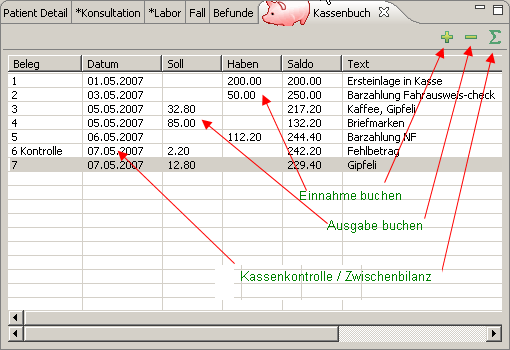
\includegraphics{images/kassenbuch}
  %\caption{Toolbar / Werkzeugleiste}
  \label{fig:kassenbuch}
\end{center}
\end{figure}

\begin{itemize}
 	\item Avec l'icône[+] vous pouvez comptabiliser des entrées et avec l'icône  [ - ] les sorties.
	\item L'icône pour la somme sert pour faire un bilan actuel de l'état de caisse. Si l'état réel actuel de la caisse est plus bas que l'état comptabilisé la différence sera notée comme déficit et s'il est plus haut comme excédent. Ce blian intérmédiaire peut être fait autant de fois que vous voulez et il peut ausi être effacé.

	\item Avec un double-click sur 'comptabiliser' on peut changer l'écriture.

	\item Avec un clic droit sur une écriture un menu de contexte s'ouvre pour effacer l'écriture ou pour faire un bilan intermédiaire.

	\item Les justificatifs sont classés selon le numéro de justificatif alphanumérique. Ce numéro devait toujours commencer avec un chiffre (ce qui est toujours proposé de façon automatique)qui doit être noté sur le ticket de caisse. S'il faudra intégrer plustard encore un justificatif on peut le faire en choisissant un numéro de justificatif entre deux. Par exemple on introduit 2a entre 2 et 3. 
\end{itemize}


